We compare FANTOM to CASTOR \citep{rahmanicausal} and KCP \citep{arlot2019kernel} in the task of regime detection. KCP is a multiple change-point detection method designed to handle univariate, multivariate, or complex data. Being non-parametric, KCP does not necessitate knowing the true number of change points in advance. It detects abrupt changes in the complete distribution of the data by employing a characteristic kernel. 

CASTOR is a causal discovery model specifically designed for multi-regime MTS. CASTOR is learns number of regime and their indices and their corresponding causal graphs without any prior knowledge. But it is limited to normal noise with equivariance. FANTOM learns the regime indices, while handling heteroscedastic noises.

We opted to perform regime detection with 10 nodes and three different regimes. For a fair comparison, we chose three regimes without re-occurrence, as KCP only detect change points and cannot identify the re-occurrence of a specific regime. 

Regarding the models employed, we use the open-source code of CASTOR implemented in Python by the authors\footnote{\url{https://github.com/arahmani1/CASTOR}}. For KCP, we employ the \texttt{Rupture} package\footnote{\url{https://centre-borelli.github.io/ruptures-docs/}}.

\begin{figure}[H]

\begin{center}
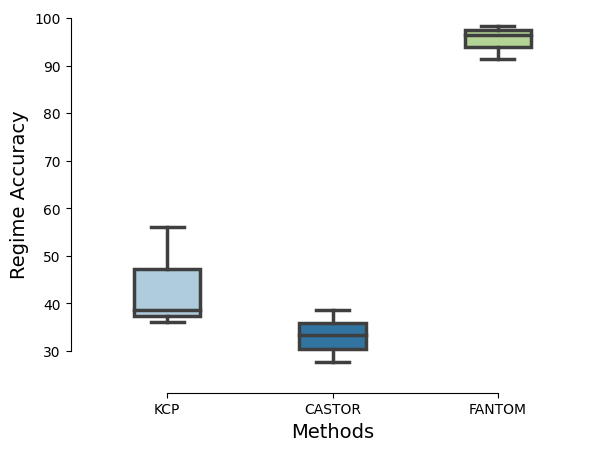
\includegraphics[width=0.7\textwidth]{figures/regime_acc_kcp_fantom.png}
\end{center}
\caption{Comparison between FANTOM, CASTOR and KCP on regime detection for a MTS with heteroscedastic noise and composed of 3 regimes using accuracy metric. The number of nodes is $d=10$.}
\label{reg_acc_fantomvskcp}
\end{figure}

From Figure \ref{reg_acc_fantomvskcp}, it is evident that FANTOM outperform CASTOR and the change-point detection method KCP. This outcome can be attributed to the limitation of KCP in detecting changing points within causal mechanisms that are represented by conditional distributions. FANTOM outperforms CASTOR in detecting regime indices. This result can be explained by the fact that CASTOR fails in handling heteroscedastic noises and fails to learn meaningful graphs which also lead to poor performance in regime detection.

From this analysis and the other experiments shown in the different tables, we can conclude that in scenarios involving MTS with multiple regimes with non-Gaussian or Heteroscedastic noises, FANTOM offers a robust solution. Additionally, employing other methods to split the regimes and learn the causal graph through traditional causal discovery methods may not be an optimal solution:
\begin{itemize}
    \item We demonstrate that regime indices are not well recoverable by other state-of-the-art change point detection method KCP. Therefore, employing KCP to learn the regimes and subsequently using methods like DYNOTEARS, PCMCI+, or Rhino to learn the graph may not constitute an optimal solution.
    \item In cases of regime recurrence, the aforementioned methods are unable to accurately detect the exact number of regimes. Therefore, if a user employs KCP and subsequently uses the regime partitions revealed by KCP as an input to a causal discovery method (such as PCMCI+, DYNOTEARS, Rhino, etc.), the running time will be significantly high.\\
    \item We show throughout all our experiments, that FANTOM outperforms all causal discovery method in DAG learning task, even when these models are in more favorable scenarios, by having access to the regime labels beforehand.
   
\end{itemize}